\documentclass[
	% -- opções da classe memoir --
	12pt,				% tamanho da fonte
	openright,			% capítulos começam em pág ímpar (insere página vazia caso preciso)
	oneside,			% para impressão em recto e verso. Oposto a oneside
	a4paper,			% tamanho do papel.
	% -- opções da classe abntex2 --
	%chapter=TITLE,		% títulos de capítulos convertidos em letras maiúsculas
	%section=TITLE,		% títulos de seções convertidos em letras maiúsculas
	%subsection=TITLE,	% títulos de subseções convertidos em letras maiúsculas
	%subsubsection=TITLE,% títulos de subsubseções convertidos em letras maiúsculas
	% -- opções do pacote babel --
	english,			% idioma adicional para hifenização
	english				% o último idioma é o principal do documento
	]{abntex2}

% ---
% Pacotes básicos
% ---
\usepackage{lmodern}			% Usa a fonte Latin Modern
\usepackage[T1]{fontenc}		% Selecao de codigos de fonte.
\usepackage[utf8]{inputenc}		% Codificacao do documento (conversão automática dos acentos)
\usepackage{indentfirst}		% Indenta o primeiro parágrafo de cada seção.
\usepackage{color}				% Controle das cores
\usepackage{graphicx}			% Inclusão de gráficos
\usepackage{microtype} 			% para melhorias de justificação
\usepackage{epigraph}
\usepackage{tcolorbox}
\usepackage{hyperref}
\usepackage{pgfgantt}
\usepackage{booktabs}
\usepackage{multirow}
\usepackage{tikz}
\usepackage{enumitem}
\usepackage{amsmath}
\usepackage{amssymb}
\usepackage{amsfonts}
\usepackage{caption}
\usepackage{subcaption}
\usepackage{circuitikz}
\usepackage{algorithm2e}
\RestyleAlgo{ruled}
\usetikzlibrary{chains, positioning, shadows, arrows.meta, calc, shapes.geometric}
\tikzset{
    block/.style={
        rectangle,
        rounded corners,
        draw=black, thick,
        text width=4.5em,
        minimum height=3em,
        align=center
    },
    arrow/.style={->, thick}
}

\usepackage[table]{xcolor}
% ---

% ---
% Pacotes adicionais, usados apenas no âmbito do Modelo Canônico do abnteX2
% ---
\usepackage{lipsum}				% para geração de dummy text
% ---

% ---
% Pacotes de citações
% ---
\usepackage[english,hyperpageref]{backref}	 % Paginas com as citações na bibl
\usepackage[alf]{abntex2cite}	% Citações padrão ABNT

%% CBM: pacote para incluir a ficha catalográfica como pdf
\usepackage[final]{pdfpages}

% ---
% CONFIGURAÇÕES DE PACOTES
% ---

% ---
% Configurações do pacote backref
% Usado sem a opção hyperpageref de backref
\renewcommand{\backrefpagesname}{Citado na(s) página(s):~}
% Texto padrão antes do número das páginas
\renewcommand{\backref}{}
% Define os textos da citação
\renewcommand*{\backrefalt}[4]{
	\ifcase #1 %
		Nenhuma citação no texto.%
	\or
		Citado na página #2.%
	\else
		Citado #1 vezes nas páginas #2.%
	\fi}%
% ---

% ---
% Informações de dados para CAPA e FOLHA DE ROSTO
% ---
\titulo{AIware: An Embedded AI System for Real-Time Driver State Monitoring and Alerting}
\autor{Antônio Nigro Zamur \\
Gabriel Pereira de Carvalho \\
Henrique Eduardo dos Santos de Souza \\
Mateus Kosicov Perugini}
\local{São Paulo, SP}
\data{2026}
\instituicao{%
  \textbf{PCS3848 - Sistemas Embarcados}
  \par
  Universidade de São Paulo -- USP
  \par
  Escola Politécnica
  \par
  Departamento de Engenharia de Computação e Sistemas Digitais (PCS)}
\tipotrabalho{}
% O preambulo deve conter o tipo do trabalho, o objetivo,
% o nome da instituição e a área de concentração
\preambulo{}
% ---


% ---
% Configurações de aparência do PDF final

% alterando o aspecto da cor azul
\definecolor{blue}{RGB}{41,5,195}

% informações do PDF
\makeatletter
\hypersetup{
     	%pagebackref=true,
		pdftitle={\@title},
		pdfauthor={\@author},
    	pdfsubject={\imprimirpreambulo},
	    pdfcreator={LaTeX with abnTeX2},
		pdfkeywords={abnt}{latex}{abntex}{abntex2}{trabalho acadêmico},
		colorlinks=true,       		% false: boxed links; true: colored links
    	linkcolor=blue,          	% color of internal links
    	citecolor=blue,        		% color of links to bibliography
    	filecolor=magenta,      		% color of file links
		urlcolor=blue,
		bookmarksdepth=4
}
\makeatother
% ---

% ---
% Posiciona figuras e tabelas no topo da página quando adicionadas sozinhas
% em um página em branco. Ver https://github.com/abntex/abntex2/issues/170
\makeatletter
\setlength{\@fptop}{5pt} % Set distance from top of page to first float
\makeatother
% ---

% ---
% Possibilita criação de Quadros e Lista de quadros.
% Ver https://github.com/abntex/abntex2/issues/176
%
\newcommand{\quadroname}{Quadro}
\newcommand{\listofquadrosname}{Lista de quadros}

\newfloat[chapter]{quadro}{loq}{\quadroname}
\newlistof{listofquadros}{loq}{\listofquadrosname}
\newlistentry{quadro}{loq}{0}

% configurações para atender às regras da ABNT
\setfloatadjustment{quadro}{\centering}
\counterwithout{quadro}{chapter}
\renewcommand{\cftquadroname}{\quadroname\space}
\renewcommand*{\cftquadroaftersnum}{\hfill--\hfill}

\setfloatlocations{quadro}{hbtp} % Ver https://github.com/abntex/abntex2/issues/176
% ---

% ---
% Espaçamentos entre linhas e parágrafos
% ---

% O tamanho do parágrafo é dado por:
\setlength{\parindent}{1.3cm}

% Controle do espaçamento entre um parágrafo e outro:
\setlength{\parskip}{0.2cm}  % tente também \onelineskip

% ---
% compila o indice
% ---
\makeindex
% ---

% ----
% Início do documento
% ----
\begin{document}

% Seleciona o idioma do documento (conforme pacotes do babel)
\selectlanguage{english}
%\selectlanguage{brazil}

% Retira espaço extra obsoleto entre as frases.
\frenchspacing

% ----------------------------------------------------------
% ELEMENTOS PRÉ-TEXTUAIS
% ----------------------------------------------------------
% \pretextual

% ---
% Capa
% ---
\imprimircapa
% ---

% ---
% Folha de rosto
% (o * indica que haverá a ficha bibliográfica)
% ---
\imprimirfolhaderosto*
% ---

% ---
% Inserir a ficha bibliografica
% ---

% Isto é um exemplo de Ficha Catalográfica, ou ``Dados internacionais de
% catalogação-na-publicação''. Você pode utilizar este modelo como referência.
% Porém, provavelmente a biblioteca da sua universidade lhe fornecerá um PDF
% com a ficha catalográfica definitiva após a defesa do trabalho. Quando estiver
% com o documento, salve-o como PDF no diretório do seu projeto e substitua todo
% o conteúdo de implementação deste arquivo pelo comando abaixo:
%
%% TODO: utilizar a ficha catalográfica gerada em https://www.poli.usp.br/bibliotecas/servicos/catalogacao-na-publicacao
%\begin{fichacatalografica}
%    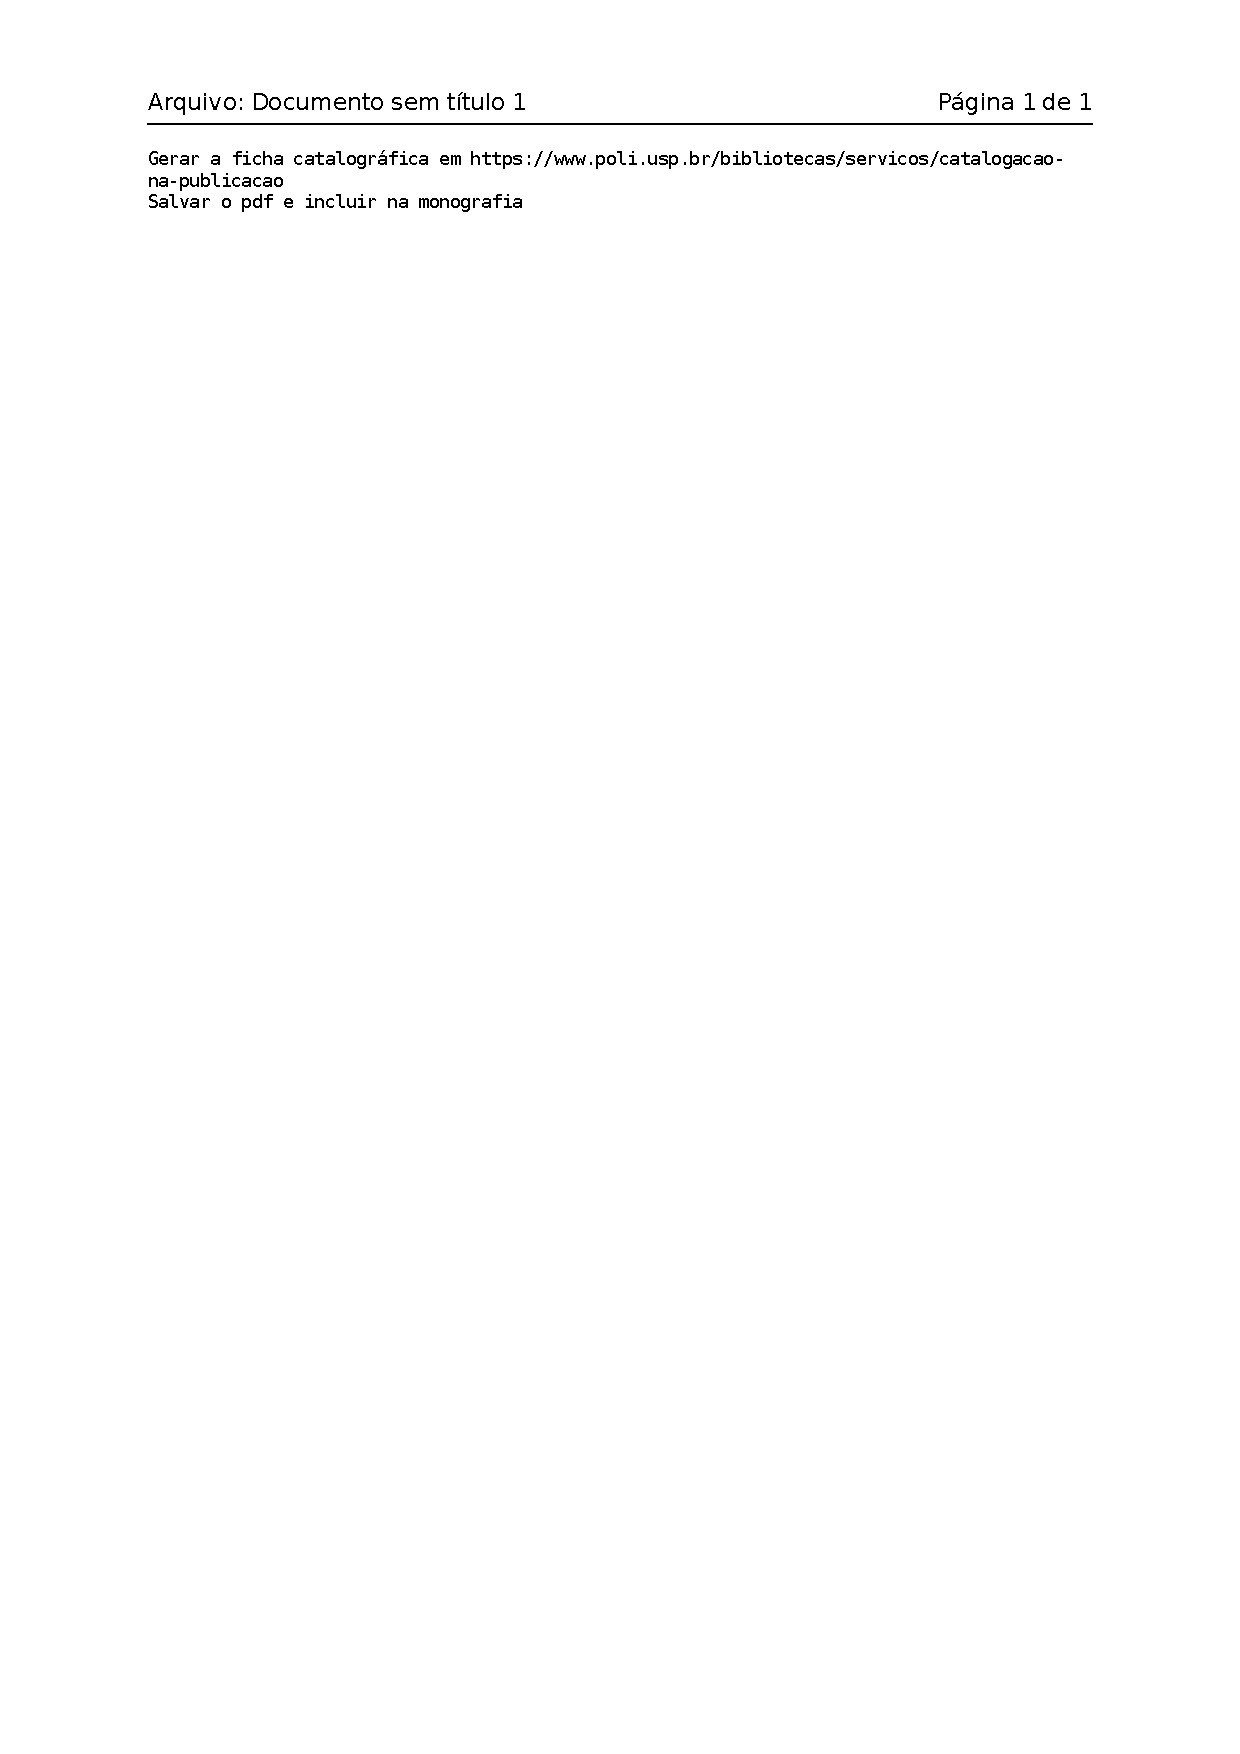
\includepdf{ficha.pdf}
%\end{fichacatalografica}

% \begin{fichacatalografica}
% 	\sffamily
% 	\vspace*{\fill}					% Posição vertical
% 	\begin{center}					% Minipage Centralizado
% 	\fbox{\begin{minipage}[c][8cm]{13.5cm}		% Largura
% 	\small
% 	\imprimirautor
% 	%Sobrenome, Nome do autor

% 	\hspace{0.5cm} \imprimirtitulo  / \imprimirautor. --
% 	\imprimirlocal, \imprimirdata-

% 	\hspace{0.5cm} \thelastpage p. : il. (algumas color.) ; 30 cm.\\

% 	\hspace{0.5cm} \imprimirorientadorRotulo~\imprimirorientador\\

% 	\hspace{0.5cm}
% 	\parbox[t]{\textwidth}{\imprimirtipotrabalho~--~\imprimirinstituicao,
% 	\imprimirdata.}\\

% 	\hspace{0.5cm}
% 		1. Palavra-chave1.
% 		2. Palavra-chave2.
% 		3. Palavra-chave3.
% 		I. Orientador.
% 		II. Universidade xxx.
% 		III. Faculdade de xxx.
% 		IV. Título
% 	\end{minipage}}
% 	\end{center}
% \end{fichacatalografica}
% ---

% ---
% Inserir folha de aprovação
% ---

% Isto é um exemplo de Folha de aprovação, elemento obrigatório da NBR
% 14724/2011 (seção 4.2.1.3). Você pode utilizar este modelo até a aprovação
% do trabalho. Após isso, substitua todo o conteúdo deste arquivo por uma
% imagem da página assinada pela banca com o comando abaixo:
%
% \begin{folhadeaprovacao}
% \includepdf{folhadeaprovacao_final.pdf}
% \end{folhadeaprovacao}
%
% \begin{folhadeaprovacao}

%   \begin{center}
%     {\ABNTEXchapterfont\large\imprimirautor}

%     \vspace*{\fill}\vspace*{\fill}
%     \begin{center}
%       \ABNTEXchapterfont\bfseries\Large\imprimirtitulo
%     \end{center}
%     \vspace*{\fill}

%     \hspace{.45\textwidth}
%     \begin{minipage}{.5\textwidth}
%         \imprimirpreambulo
%     \end{minipage}%
%     \vspace*{\fill}
%    \end{center}

%    Trabalho aprovado. \imprimirlocal, 24 de novembro de 2012:

%    \assinatura{\textbf{\imprimirorientador} \\ Orientador}
%    \assinatura{\textbf{Professor} \\ Convidado 1}
%    \assinatura{\textbf{Professor} \\ Convidado 2}
%    %\assinatura{\textbf{Professor} \\ Convidado 3}
%    %\assinatura{\textbf{Professor} \\ Convidado 4}

%    \begin{center}
%     \vspace*{0.5cm}
%     {\large\imprimirlocal}
%     \par
%     {\large\imprimirdata}
%     \vspace*{1cm}
%   \end{center}

% \end{folhadeaprovacao}
% ---

% ---
% Dedicatória
% ---
%\begin{dedicatoria}
%   \vspace*{\fill}
%   \centering
%   \noindent
%   \textit{"The prize is in the pleasure of finding the thing out."} \\ \raggedleft{\textit{Richard P. Feynman}} \vspace*{\fill}
   %\textit{"I saw the angel in the marble and carved until I set him free."} \\ \raggedleft{\textit{Michelangelo}} \vspace*{\fill}
   %\textit{"Maybe I had a secret identity, but then when you think about it, don't we all? A part of ourselves very few people ever get to see. The part we think of as "me". The part that deals with the big stuff. Makes the real choices. The part everything else is a reflection of."} \\ \raggedleft{\textit{Kurt Busiek, Superman - Secret Identity \#4}} \vspace*{\fill}
%\end{dedicatoria}
% ---

% ---
% Agradecimentos
% ---
%\begin{agradecimentos}
%...
%\end{agradecimentos}
% ---

% ---
% Epígrafe
% ---
% \begin{epigrafe}
%     \vspace*{\fill}
% 	\begin{flushright}
% 		\textit{...}
% 	\end{flushright}
% \end{epigrafe}
% ---

% ---
% RESUMOS
% ---

% resumo em português
\setlength{\absparsep}{18pt} % ajusta o espaçamento dos parágrafos do resumo
\begin{resumo}[Resumo]
Apresentamos o projeto do nosso grupo: AIware, um sistema de inteligência artificial embarcada para monitoramento e alerta do estado do condutor em tempo real. Nossa proposta de projeto visa enfrentar o problema dos acidentes de trânsito causados por fadiga e distração por meio de uma solução de baixo custo e alta eficiência. A proposta foca no estudo de trabalhos relacionados explorando modelos de Deep Learning compactos (TinyML) e como otimizá-los para hardware com recursos limitados

 \textbf{Palavras-chave}: Embedded AI. TinyML. Driver Monitoring Systems (DMS).
\end{resumo}

% resumo em inglês
\begin{resumo}[Abstract]
 \begin{otherlanguage*}{english}
   We present our group's project: AIware, an embedded artificial intelligence system for real-time driver state monitoring and alerting. Our project proposal aims to tackle the problem of traffic accidents caused by fatigue and distraction through a low-cost, high-efficiency solution. The proposal focuses on the study of related works exploring tiny Deep Learning models optimized for resource-constrained hardware.

   \vspace{\onelineskip}

   \noindent
   \textbf{Keywords}: Embedded AI. TinyML. Driver Monitoring Systems (DMS).
 \end{otherlanguage*}
\end{resumo}

% % resumo em francês
% \begin{resumo}[Résumé]
%  \begin{otherlanguage*}{french}
%     Il s'agit d'un résumé en français.

%    \textbf{Mots-clés}: latex. abntex. publication de textes.
%  \end{otherlanguage*}
% \end{resumo}

% % resumo em espanhol
% \begin{resumo}[Resumen]
%  \begin{otherlanguage*}{spanish}
%    Este es el resumen en español.

%    \textbf{Palabras clave}: latex. abntex. publicación de textos.
%  \end{otherlanguage*}
% \end{resumo}
% ---

% ---
% inserir lista de ilustrações
% ---
%\pdfbookmark[0]{\listfigurename}{lof}
%\listoffigures*
%\cleardoublepage
% ---

% ---
% inserir lista de quadros
% ---
%\pdfbookmark[0]{\listofquadrosname}{loq}
%\listofquadros*
%\cleardoublepage
% ---

% ---
% inserir lista de tabelas
% ---
%\pdfbookmark[0]{\listtablename}{lot}
%\listoftables*
%\cleardoublepage
% ---

% ---
% inserir lista de abreviaturas e siglas
% ---
%\begin{siglas}
%  \item[ABNT] Associação Brasileira de Normas Técnicas
%  \item[abnTeX] ABsurdas Normas para TeX
%\end{siglas}
% ---

% ---
% inserir lista de símbolos
% ---
%\begin{simbolos}
%  \item[$ \Gamma $] Letra grega Gama
%  \item[$ \Lambda $] Lambda
%  \item[$ \zeta $] Letra grega minúscula zeta
%  \item[$ \in $] Pertence
%\end{simbolos}
% ---

% ---
% inserir o sumario
% ---
%\pdfbookmark[0]{\contentsname}{toc}
\tableofcontents*
%\cleardoublepage
% ---


% ----------------------------------------------------------
% ELEMENTOS TEXTUAIS
% ----------------------------------------------------------
\textual

% Capítulo 1. Introdução
\chapter{Introduction} \label{cap:introducao}

%Este documento é baseado no exemplo de referência de uso da classe
%\textsf{abntex2} e do pacote \textsf{abntex2cite}.
%Este documento é uma referência e os manuais do \abnTeX\ \cite{abntex2classe,abntex2cite,abntex2cite-alf} e da classe \textsf{memoir} \cite{memoir} possuem informações completas.

%(Observe no parágrafo anterior como são feitas as citações! As referências estão no arquivo abntex2-modelo-references.bib, seguindo um formato específico para as informações necessárias. Ah, se você quiser fazer uma citção com o nome do autor no meio do texto, por exemplo dizendo que o \citeonline{abntex2classe} fez um trabalho importante, você usa o citeonline).

%Os capítulo, seções e conteúdos aqui propostos são baseados no documento \textit{Sumário para Monografia de Projeto de Formatura}.

%% CONTEXT
\section{Context}

%%%%%%%%%%%%%%%%%%%%%%%%%%
\section{Motivation}

%\begin{itemize}
%    \item Apresentar o estado de arte resumido do assunto que será o tema do desenvolvimento do trabalho, elaborado com base nos trabalhos consultados.
%    \item Citar os trabalhos consultados no texto.
%    \item Contexto em que o trabalho será desenvolvido.
%\end{itemize}

%%%%%%%%%%%%%%%%%%%%%%%%%%
\section{Objectives}

%\begin{itemize}
%    \item Apresentar o objetivo do trabalho de forma precisa e concisa.
%    \item O que é o trabalho?
%\end{itemize}

%%%%%%%%%%%%%%%%%%%%%%%%%%

%%%%%%%%%%%%%%%%%%%%%%%%%%
\section{Related works}

%\begin{itemize}
%    \item Apresentar porque o trabalho desenvolvido é importante (importância e necessidade para a sociedade, comparação com trabalhos relevantes consultados etc.).
%    \item Citar os trabalhos consultados no texto.
%    \item Por que o trabalho é importante?
%\end{itemize}

%%%%%%%%%%%%%%%%%%%%%%%%%%
\section{Organisation}

%Descrever sucintamente os capítulos e as demais partes do trabalho.
%Lembre-se de colocar rótulos nos capítulos e seções (com label{} ) e depois utilizar o ref{}
%Por exemplo, o Capítulo \ref{cap:conceitos} apresenta conceitos....




% Capítulo 2. Aspectos Conceituais
\chapter{Camera-Based Driver Monitoring} \label{cap:conceitos}

%\begin{itemize}
%    \item Definir as seções representativas em função do trabalho.
%    \item Apresentar os conceitos empregados e a revisão da literatura.
%    \item Citar os trabalhos consultados no texto.
%\end{itemize}

In this chapter, we introduce some interesting concepts analysed by the group when studying literature for camera-based driver monitoring systems.

\section{Near-Infrared (NIR) Imaging}

One of the primary challenges faced in the camera-based approach is maintaining consistent performance under varying lighting conditions, such as driving at night or through tunnels. According to \cite{review}, Near-Infrared (NIR) imaging is the standard solution to this problem. Unlike standard RGB cameras, NIR systems operating in the $850--940$ nanometer can capture facial features in total darkness. In our AIware project, if using an infrared camera is not possible, we can try to incorporate microphone-based based to help our model make good predictions even when image quality is suboptimal.

\section{Behavioral Biometrics: EAR and MAR Metrics}

To objectively quantify driver states like drowsiness and distraction, two of the most critical metrics are the Eye Aspect Ratio (EAR) and the Mouth Aspect Ratio (MAR).
\begin{itemize}
    \item \textbf{EAR} monitors the distance between eyelids to detect blinks and prolonged eye closure (micro-sleeps).
    \item \textbf{MAR} measures mouth opening levels to identify frequent yawning, a primary indicator of early-stage fatigue.
\end{itemize}

\begin{figure}[h!]
    \centering
    \caption{Eye Aspect Ratio metric \cite{bellino2018}}
    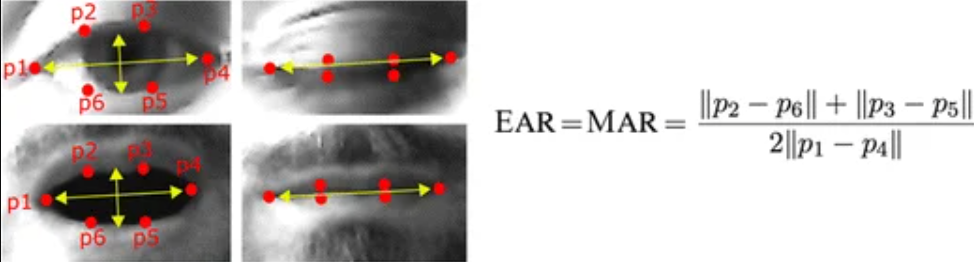
\includegraphics[width=.7\textwidth]{images/EAR.png}
    \label{fig:ear}
\end{figure}

\begin{figure}[h!]
    \centering
    \caption{Mouth Aspect Ratio metric \cite{zhu2022}}
    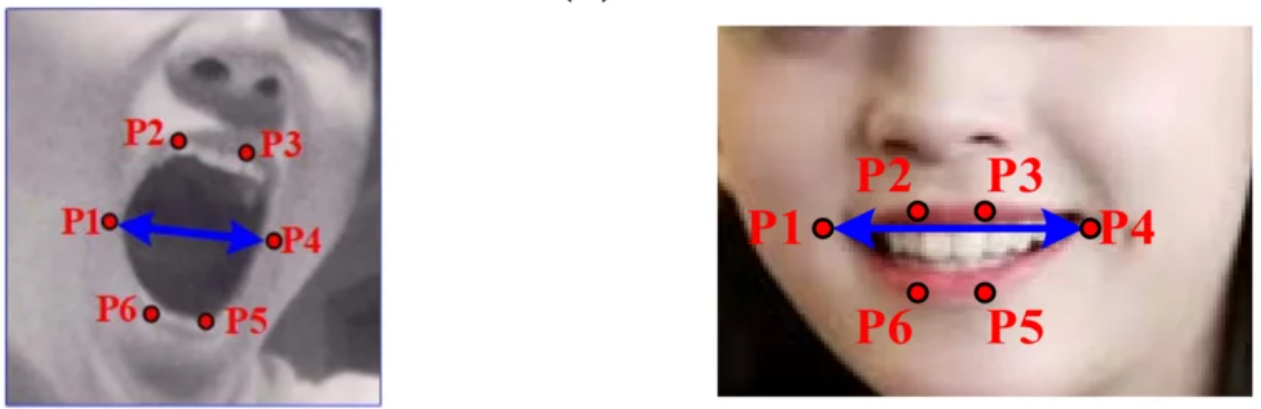
\includegraphics[width=.7\textwidth]{images/MAR.png}
    \label{fig:mar}
\end{figure}


According to \cite{review}, these geometric ratios allow lightweight AI models to perform binary classifications with high precision and low computational overhead, fitting the constraints of edge devices.

\section{Remote Photoplethysmography (rPPG)}

A more advanced concept discussed in recent literature is remote Photoplethysmography (rPPG), which allows for the detection of physiological signals such as heart rate and respiration using only a standard camera sensor. By analyzing minute skin color variations caused by blood circulation (which are often imperceptible to the human eye), the system can infer the driver's stress levels or sudden health emergencies. This is a very interesting technique, however it is unlike we will explore it for the AIware project in the Embedded Systems Laboratory course.

% Capítulo 3. Metodologia do Trabalho
%\include{Cap3-Metodo}

% Capítulo 4. Especificação de Requisitos
\chapter{Project Requirement Specification} \label{cap:especificacao}

%Definir e descrever os requisitos do sistema.



% Capítulo 5. Desenvolvimento do Trabalho
\chapter{Project Architecture} \label{cap:desenvolvimento}

In this chapter, we translate the listed requirements into a selection of specific components to constitute the final system. The primary platform for implementing the artificial intelligence models will be a Raspberry Pi 3B+. The device features 1GB of RAM, which is expected to be sufficient for executing lightweight AI models following preliminary image processing. For prototyping purposes, an OV7670 camera with 300KP resolution (currently owned by a member of the group) may be used; however, if available in the laboratory the final product is intended to utilize a camera with a minimum resolution of 2MP.

\begin{figure}[h!]
    \centering
    \caption{Block diagram with the AIware system architecture}
    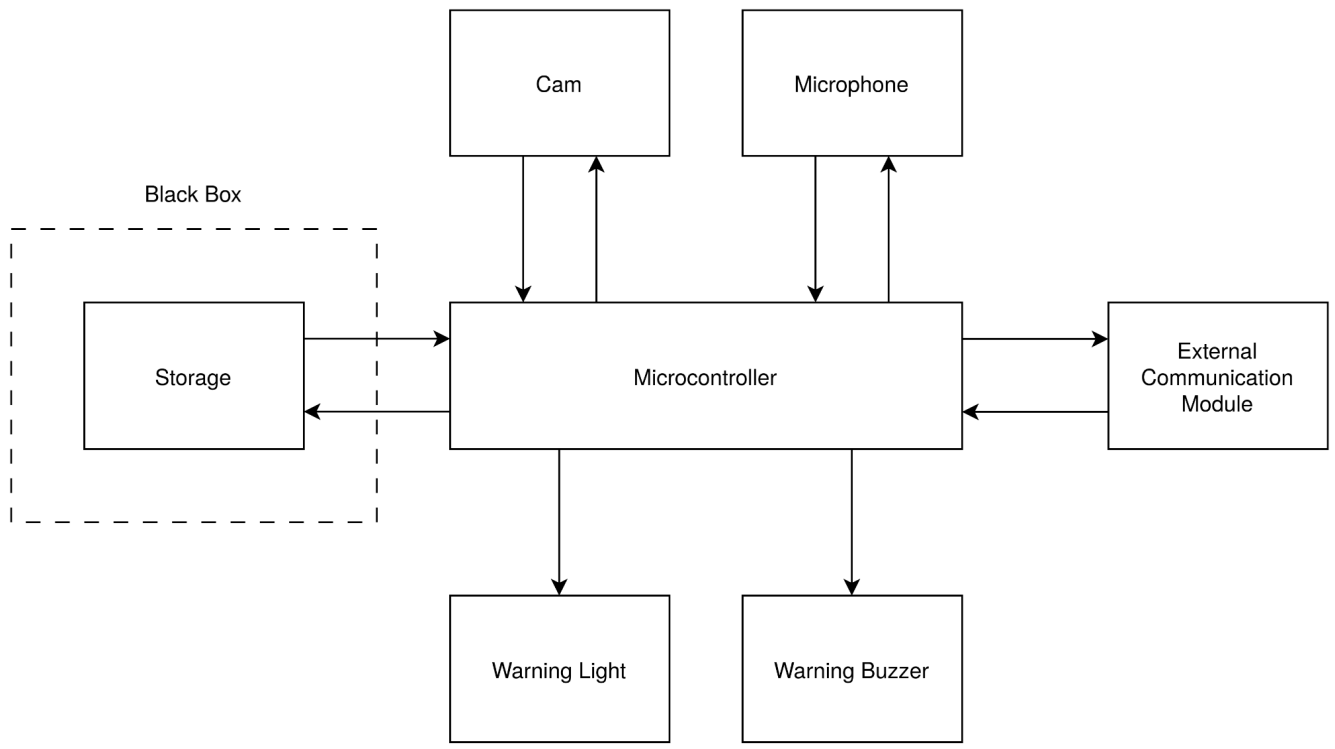
\includegraphics[width=.9\textwidth]{images/architecture.png}
    \label{fig:arch}
\end{figure}

To generate the audible alert, a standard 5V active buzzer will be employed, as it is capable of emitting approximately 85dB at a distance of 10cm, ensuring effectiveness given the system's proximity to the driver. Regarding the visual alert signal, 5mm LEDs are considered for the prototyping phase, with the potential transition to a high-intensity light source for the final version to meet the required luminance specifications.

Regarding external communication, the system implements the MQTT (Message Queuing Telemetry Transport) protocol to transmit driver state and telemetry data to the central monitoring hub. By using MQTT, the AIware system can send periodic updates with minimal protocol overhead, reducing both latency and bandwidth consumption. Furthermore, the protocol's Quality of Service (QoS) levels allow the system to prioritize critical event notifications such as the detection of severe fatigue or a medical emergency ensuring that these alerts are acknowledged by the central server even if the connection is momentarily interrupted.

Initially, LoRa was considered as a possible alternative in our group discussions because of the low volume, low energy consumption and because LoRa stations can cover big distances. However, we opted for MQTT in the end because LoRa requires a dedicated network of gateways. Since a vehicle is mobile and may travel across cities or highways, relying on a provider's private LoRa network is impractical. Using the existing Cellular Network via MQTT seems like a simpler and more straightforward solution.


% ----------------------------------------------------------
% Finaliza a parte no bookmark do PDF
% para que se inicie o bookmark na raiz
% e adiciona espaço de parte no Sumário
% ----------------------------------------------------------
\phantompart

% ---
% Conclusão
% ---
% Capítulo 6. Considerações Finais
%\chapter{Conclusions} \label{cap:consideracoes}

In this monograph we presented the activities we developed in the course and some of the study materials we reviewed. With this project proposal for the Alware system, we studied topics in the intersection of safety analysis and embedded AI.

The literature review provided an encouraging outlook for the project's feasibility. Using TinyML architectures, high-accuracy driver state detection is achievable even on resource-constrained hardware \cite{essa2026} \cite{lumina2026}.

A significant portion of this study was dedicated to the project requirement specification and architecture. Moving forward into the Embedded Systems Laboratory course, our focus will shift from theoretical specification to practical development. This will include model training and optimization using TensorFlow Lite to compress deep learning models for the Raspberry Pi environment; physical integration of the camera to ensure good quality a real-time image data stream; and assembling the black box enclosure, ensuring the buzzer and LED alerts meet the specified intensity requirements for driver engagement.

In summary, while this is an initial study, the clarity of the requirements and the efficiency of the proposed architecture suggest that Alware is a feasible solution for enhancing driver safety through low-cost, high-efficiency embedded AI.

% ----------------------------------------------------------
% ELEMENTOS PÓS-TEXTUAIS
% ----------------------------------------------------------
\postextual
% ----------------------------------------------------------

% ----------------------------------------------------------
% Referências bibliográficas
% ----------------------------------------------------------
\bibliography{abntex2-modelo-references}

%---------------------------------------------------------------------
% INDICE REMISSIVO
%---------------------------------------------------------------------
\phantompart
\printindex
%---------------------------------------------------------------------

\end{document}